\documentclass[letterpaper,12pt,oneside]{book}
%\usepackage[a4paper,includeall,bindingoffset=0cm,margin=2cm,marginparsep=0cm,marginparwidth=0cm]{geometry}
%\usepackage[top=1in, left=0.9in, right=1.25in, bottom=1in]{geometry}
%\usepackage{bachelorstitlepageUNAM}
\usepackage{ragged2e}
\usepackage{times}
\usepackage{listings}
\usepackage{xcolor}
%\usepackage{background}
\usepackage[utf8]{inputenc}
\usepackage{url}
\usepackage[T1]{fontenc}
\usepackage[spanish,es-nodecimaldot,es-tabla]{babel}
\usepackage{graphicx}
\usepackage{tikz}
\usepackage{tocloft}
\graphicspath{{./figs/}}
\usepackage{setspace}
\usepackage{comment}
\usepackage{hyperref}
\urlstyle{same}
\hypersetup{
   colorlinks=true,
   urlcolor=cyan,
   linkcolor=black,
   citecolor=black,
   filecolor=magenta,
   pdftitle={Sharelatex Example},
   pdfpagemode=FullScreen,
}
\usepackage[natbibapa]{apacite}
%\usepackage[round]{natbib}

%\renewcommand\cftsecpresnum{\S}
%\renewcommand\cftsubsecpresnum{\S}

%%%%%%%%%%%%%%%%%%%%%%%%%%%%%

% Modificación de la plantilla original de esta url: 
% https://es.overleaf.com/latex/templates/tesis-unam-ingenieria-energia/kfffjrxcckdp

% Adaptada por Carlos Rodríguez Díaz para el CIC IPN.
% Cualquier sugerencia, corrección o comentario a: amnet04@gmail.com

% A continuación los comentarios de la plantilla original:

% Comparto una plantilla para la PORTADA que us\'e en mi t\'esis
% basada en el dise\~no gen\'erico que se usa en la Facultad de Ciencias
% Para usarlo \'unicamente aseg\'urate de tener la l\'inea
% \usepackage{bachelorstitlepageUNAM} y el archivo bachelorstitlepageUNAM.sty en el mismo directorio de trabajo.
% y los campos (sin signo %) :
%\author{Nombre del Alumno}
%\title{T\'itulo de la tesis}
%\faculty{Facultad}
%\degree{Grado que obtienes}
%\supervisor{ Tutor}
%\cityandyear{Ciudad y anio}
%\logouni{nombredelescudodelaunamsinespacios}
%\logofac{NombreDeLaImagenDelEscudodeTuFacultadSinEspacios}
% Para sugerencias y comentarios: DM en twitter.com/sglvgdor
% Subir\'e mas adelante la plantilla para maestr\'ia
%%%%%%%%%%%%%%%%%%%%%%%%%%%%%


\begin{document}

\frontmatter
            \begin{titlepage}
  \thispagestyle{empty}
  \begin{minipage}[c][0.17\textheight][c]{0.25\textwidth}
    \begin{center}
      
\includegraphics[ height=4cm]{Images/logo-ipn.png}
    \end{center}
  \end{minipage}
  \begin{minipage}[c][0.195\textheight][t]{0.75\textwidth}
    \begin{center}
      \vspace{0.3cm}
             {\color{red}\textsc{\large Instituto Politécnico Nacional} }\\[0.5cm]
             \vspace{0.3cm}
                    {\color{purple}\hrule height2.5pt}
                    \vspace{.2cm}
                           {\color{purple}\hrule height1pt}
                           \vspace{.8cm}
                           \textsc{Escuela Superior de Cómputo }\\[1cm] %
    \end{center}
  \end{minipage}
  \begin{minipage}[c][0.81\textheight][t]{0.25\textwidth}
    \vspace*{5mm}
    \begin{center}
      \hskip2.0mm
             {\color{red}\vrule width1pt height13cm }
             \vspace{5mm}
             \hskip2pt
                 {\color{red}\vrule width2.5pt height13cm}
                 \hskip2mm
                     {\color{red}\vrule width1pt height13cm} \\
                     \vspace{5mm}
                     
\includegraphics[height=3.0cm]{Images/CIC.png}
    \end{center}
  \end{minipage}
  \begin{minipage}[c][0.81\textheight][t]{0.75\textwidth}
    \begin{center}
      \vspace{1cm}

      {\color{red}{\large\scshape Titulo del Reporte }}\\[.2in]

      \vspace{2cm}            

      \textsc{\LARGE P\hspace{0.5cm}R\hspace{0.5cm}O\hspace{0.5cm}G\hspace{0.5cm}R\hspace{0.5cm}A\hspace{0.5cm}M\hspace{0.5cm}A\hspace{0.5cm}}\\[1cm]
      \textsc{\LARGE A\hspace{0.5cm}U\hspace{0.5cm}T\hspace{0.5cm}Ó\hspace{0.5cm}M\hspace{0.5cm}A\hspace{0.5cm}T\hspace{0.5cm}A}\\[1cm]
      \textsc{\LARGE  \hspace{0.5cm}D\hspace{0.5cm}E}\\[1cm]
      \textsc{\LARGE\hspace{0.5cm}P\hspace{0.5cm}I\hspace{0.5cm}L\hspace{0.5cm}A}
      \\[1cm]
      \textsc{\large para obtener un 10 en el reporte:}\\[0.2cm]
     % \textsc{\large XXXX XXXX XXXXX}\\[0.5cm]
      
      {\color{red}\textsc{\large presenta:}}\\[0.2cm]
      \textsc{\large {Connor Urbano Mendoza}}\\[1cm]          

      \vspace{0.5cm}

      {\large\scshape 
        {\color{red}Docentes:}\\[0.3cm] {Juárez Martínez Genaro}}\\[.2in]

      \vspace{1cm}

      \large{Estados Unidos Mexicanos\\ 
        Ciudad de México\\
        2023}
    \end{center}
  \end{minipage}
\end{titlepage}
%---------------------------------
\tableofcontents
\listoffigures
%\chapter{Notación}


\chapter{Introducción}
Me complace presentarle el informe de mi práctica individual sobre la implementación de un autómata de pila (PDA, por sus siglas en inglés) para reconocer el lenguaje libre de contexto $[$0$^$n 1$^$n | n >= 1$]$. En esta práctica, se nos proporcionaron las instrucciones necesarias para resolver el problema planteado y se nos solicitaron ciertas características específicas para el programa.\newline

El objetivo principal de esta práctica fue diseñar y desarrollar un autómata de pila que pudiera reconocer correctamente las cadenas pertenecientes al lenguaje $[$0$^$n 1$^$n | n >= 1$]$. Además, se nos pidió implementar ciertas funcionalidades adicionales para enriquecer la experiencia del usuario y facilitar la evaluación del autómata.\newline

Las características solicitadas para el programa fueron las siguientes:\newline

\begin{enumerate}
\item La posibilidad de que el usuario ingrese la cadena manualmente o que sea generada automáticamente. En el segundo caso, se estableció como requisito que la cadena no pudiera exceder los 100,000 caracteres.\newline

\item La generación de un archivo y la visualización en pantalla de las descripciones instantáneas (IDs) correspondientes a la evaluación del autómata. Esta función permitirá analizar paso a paso el proceso de reconocimiento de la cadena ingresada.\newline

\item La animación del autómata de pila, siempre y cuando la cadena tenga una longitud menor o igual a 10 caracteres. Esta característica adicional brindará una representación visual más interactiva del funcionamiento del autómata.\newline

\item La inclusión de pantallas del programa en ejecución en el informe, mostrando todas las características solicitadas. Estas capturas de pantalla servirán para ilustrar y respaldar los resultados obtenidos durante la implementación.\newline

\item La presentación del código de la implementación en formato LaTeX, en lugar de utilizar imágenes. Esto permitirá una visualización más clara y facilitará la revisión del código.\newline

\end{enumerate}
    
A lo largo de este informe, se detallarán los pasos seguidos para cumplir con los requisitos mencionados, incluyendo el diseño del autómata, la implementación del programa en Python, el registro de las descripciones instantáneas, la animación cuando corresponda y la generación del informe en LaTeX.


\mainmatter
\chapter{Desarrollo}
\lstset{
    language=C,
    basicstyle=\ttfamily\small\color{black},
    numbers=left,
    numberstyle=\tiny,
    stepnumber=1,
    numbersep=8pt,
    backgroundcolor=\color{white},
    showspaces=false,
    showstringspaces=false,
    showtabs=false,
    frame=single,
    rulecolor=\color{magenta},
    tabsize=2,
    captionpos=b,
    breaklines=true,
    breakatwhitespace=false,
    title=\lstname,
    escapeinside={\%*}{*)},
    keywordstyle=\color{blue},
    commentstyle=\color{red},
    stringstyle=\color{orange},
    morecomment=[l][\color{red}]{\#},
    otherkeywords={=,!,<,>,*,+,-,&,|,^,~},
    numbers=left,                   % Coloca los números de línea a la izquierda
    numberstyle=\tiny\color{black}, % Estilo de los números de línea
    stepnumber=1,    % Incremento en el que se muestran los números de línea
    numbersep=8pt
}
\section{Análisis del problema principal}

%\begin{comment}
  %Objetivo: Explicarles a los lectores de computación que entienden
  %los lingüistas de una variación dialectal
%\end{comment}

%Citar a \cite{deSaussure1945}, Coseriu y Montes:

El análisis del problema principal para resolver el problema del autómata de pila se centra en comprender y abordar los siguientes aspectos clave:\newline


\begin{enumerate}

\item Lenguaje libre de contexto: El problema implica reconocer el lenguaje libre de contexto [0$^$n 1$^$n | n $>=$ 1], que consiste en cadenas formadas por una secuencia de ceros seguida de una secuencia igual de unos, con al menos un par de ceros y unos. Es fundamental comprender las reglas y características de este lenguaje para diseñar un autómata de pila adecuado.\newline

\item Autómata de pila: El autómata de pila es un modelo computacional que utiliza una pila para almacenar y procesar información durante la evaluación de una cadena. Es necesario estudiar y comprender el funcionamiento de este tipo de autómata, así como su estructura y las transiciones entre estados, con el fin de diseñar un autómata de pila que reconozca correctamente el lenguaje planteado.\newline

\item Características adicionales: Además de la implementación básica del autómata de pila, se solicitan características adicionales, como la posibilidad de ingreso manual o automático de la cadena, la generación de descripciones instantáneas (IDs) para el seguimiento del proceso de evaluación, la animación del autómata en caso de cadenas cortas y la presentación del informe en formato LaTeX. Estas características requieren un análisis adicional para determinar cómo implementarlas de manera eficiente y satisfactoria.\newline

\item Complejidad del problema: Se menciona que la cadena generada aleatoriamente no puede exceder los 100,000 caracteres. Esto implica considerar la complejidad y eficiencia del algoritmo implementado, ya que se debe garantizar que el programa sea capaz de manejar cadenas de tamaño considerable sin afectar significativamente el rendimiento.\newline
\end{enumerate}
\\

\section{Límites del problema}%seccion2

En el problema del autómata de pila, existen ciertos límites y consideraciones que debemos tener en cuenta para su resolución adecuada. Estos límites son fundamentales para garantizar el correcto funcionamiento del programa y la eficiencia en la evaluación de las cadenas ingresadas.\newline

En primer lugar, se establece un límite máximo para la longitud de la cadena. Si la cadena es generada automáticamente, se determina que no puede exceder los 100,000 caracteres. Esta restricción nos permite gestionar adecuadamente cadenas de gran tamaño, evitando posibles problemas de rendimiento y optimizando el procesamiento de la información.\newline

Por otro lado, es importante considerar el número mínimo de caracteres necesarios en la cadena. Dado que el lenguaje libre de contexto $[$0$^$n 1$^$n | n >= 1$]$ requiere que haya al menos un par de ceros seguido de un par de unos, se establece un límite mínimo de 4 caracteres. Esto garantiza que la cadena tenga la estructura necesaria para formar los pares correspondientes y cumpla con las reglas del lenguaje.\newline

Además, se solicita la animación del autómata de pila en la implementación del programa. Sin embargo, esta animación se limita a cadenas de hasta 10 caracteres. Esta restricción nos permite visualizar de manera clara y comprensible el funcionamiento del autómata, evitando la saturación de información en casos de cadenas demasiado largas.\newline


\section{Estrategia para atacar el problema}
%inicio
La estrategia para resolver el problema del autómata de pila consiste en diseñar e implementar un programa que simule el comportamiento de un autómata de pila para reconocer el lenguaje libre de contexto $[$0$^$n 1$^$n | n >= 1$]$. A continuación, se presenta una descripción general de la estrategia a seguir:\newline


\begin{enumerate}
    \item Diseño del autómata de pila: Se debe definir la estructura y el comportamiento del autómata de pila. Esto implica determinar los estados, las transiciones, los símbolos de entrada, los símbolos de pila y las reglas de transición necesarias para reconocer el lenguaje $[$0$^$n 1$^$n | n >= 1$]$. Es importante tener en cuenta las reglas específicas de este lenguaje, que requieren que el número de ceros sea igual al número de unos.\newline
    \item Implementación del programa: Se debe desarrollar el programa que simule el autómata de pila. Esto implica escribir el código en el lenguaje de programación elegido, utilizando las estructuras de datos adecuadas y siguiendo las reglas de transición definidas en el diseño del autómata.\newline
    \item Entrada de la cadena: El programa debe permitir al usuario ingresar una cadena o generarla aleatoriamente, dependiendo de las características solicitadas. En el caso de la generación aleatoria, se debe verificar que la cadena generada no exceda el límite máximo establecido.\newline
    \item Evaluación del autómata: El programa debe evaluar la cadena ingresada utilizando el autómata de pila implementado. Para ello, se aplicarán las reglas de transición correspondientes y se realizará un seguimiento de las descripciones instantáneas del autómata, que mostrarán el estado actual, los símbolos de entrada y los símbolos en la pila en cada paso.\newline
    \item Resultados y visualización: El programa debe mostrar en pantalla y guardar en un archivo las descripciones instantáneas del autómata durante la evaluación de la cadena. Además, si la longitud de la cadena es menor o igual a 10, se puede animar el autómata para una visualización más interactiva y comprensible.\newline
    
\end{enumerate}


\section{Implementación} 

Para desarrollar la implementación del problema, al autómata de pila determinista (PDA) en Python utilizando la biblioteca PIL (Python Imaging Library) para crear imágenes. El PDA en el código tiene una serie de transiciones definidas en forma de diccionario.\newline

El código se divide en dos funciones principales: proceso\_recorrido y proceso\_recorrido2. Ambas funciones reciben una cadena, un estado inicial y un índice como argumentos.\newline

La función proceso\_recorrido realiza un recorrido de la cadena en el PDA sin graficar el proceso. Muestra información relevante en la consola y escribe las transiciones en un archivo de texto.\newline

La función proceso\_recorrido2 realiza un recorrido de la cadena en el PDA y grafica el proceso en una imagen utilizando la biblioteca PIL. Dibuja rectángulos, texto y flechas para representar los diferentes estados y transiciones del PDA. También guarda la imagen generada en un archivo llamado "animacion.png".\newline

Ambas funciones utilizan el diccionario PDA para determinar las transiciones del PDA. El diccionario PDA tiene como clave una tupla que representa el estado actual, el símbolo de entrada y el símbolo en la cima de la pila, y como valor una lista de transiciones posibles. Cada transición es una tupla que contiene el estado siguiente y el símbolo que se apunta en la pila.\newline

Entrando más en detalles, iré mostrando paso a paso las partes del código:\newline


\newpage
\\

\begin{enumerate}
\item La explicación de la parte básica del código empieza por las siguientes librerías:\newline
\begin{enumerate}
    \item import random\newline
    \item from PIL import Image, ImageDraw,ImageFont\newline
    \item import sys\newline
\end{enumerate}


Las librerías random, Image, ImageDraw, ImageFont y sys son módulos de Python que brindan funcionalidades adicionales para el desarrollo de aplicaciones.\newline

La librería random proporciona funciones relacionadas con la generación de números aleatorios. Al importar esta librería, podemos utilizar métodos como random.randint() para generar números enteros aleatorios dentro de un rango específico. También podemos utilizar random.choice() para seleccionar aleatoriamente un elemento de una lista.\newline

La librería PIL (Python Imaging Library) es una biblioteca popular para el procesamiento de imágenes en Python. Al importar los módulos Image, ImageDraw y ImageFont de PIL, obtenemos funcionalidades para crear, editar y manipular imágenes. Podemos cargar imágenes existentes, crear nuevas imágenes, dibujar formas y textos en ellas, aplicar filtros y efectos, y mucho más.\newline

El módulo sys proporciona funciones y variables relacionadas con la funcionalidad del intérprete de Python y el sistema en el que se está ejecutando. Al importar este módulo, podemos acceder a variables como sys.argv, que contiene una lista de los argumentos pasados al script de Python desde la línea de comandos. También podemos utilizar sys.exit() para finalizar la ejecución del programa en cualquier momento.\newline


Se definen algunas variables iniciales, como el tamaño de la imagen y el tamaño del cuadrado para la visualización gráfica (estas variables son utilizadas más adelante para crear una imagen en blanco), así como el diccionario PDA que define las transiciones del autómata de pila.\newline

Se define la función generar\_cadena\_aleatoria(tamanio) que genera una cadena aleatoria de tamaño compuesta por los caracteres $"$0$"$ y $"$1$"$. Esta función es utilizada más adelante para generar una cadena aleatoria si el usuario no proporciona una.\newline

Se definen las funciones de recorrido 1 y recorrido 2. Estas funciones no están incluidas en el código que has proporcionado, por lo que no puedo proporcionar una explicación detallada sobre ellas.\newline

Se crea una pila vacía y se agrega el símbolo 'Z0' como elemento superior de la pila. Luego se imprime el contenido de la pila.\newline

Se solicita al usuario que ingrese una cadena de entrada. Si el usuario no ingresa ninguna cadena y simplemente presiona Enter, se genera una cadena aleatoria utilizando la función generar\_cadena\_aleatoria().\newline

Se realiza el proceso de recorrido utilizando la función proceso\_recorrido() si se generó una cadena aleatoria, o utilizando la función proceso\_recorrido2() si se ingresó una cadena manualmente. Estas funciones son responsables de validar si la cadena es válida según las reglas del autómata de pila.\newline

Dependiendo del resultado obtenido, se imprime un mensaje indicando si la cadena es válida o no.\newline

Luego, se inicia un ciclo for que recorre cada una de las palabras de la línea actual y se realiza una serie de acciones por cada palabra. En resumen, la función evalúa cada palabra en el DFA y registra las palabras encontradas en los archivos de salida, dependiendo de su categoría y su frecuencia en el texto de entrada. La parte del código que falta en el último for es probablemente la que contiene la lógica principal para evaluar cada palabra en el DFA y llevar un registro de las palabras encontradas.\newline

A continuación se presentan las partes de código correspondientes a la explicación anterior: Observar Figura 1.1.\newline
\begin{lstlisting}
#Teoria de la computacion
#Automata de pila
#Alumno: Connor Urbano Mendoza

import random
from PIL import Image, ImageDraw,ImageFont
import sys

# Tamaño de la imagen y tamaño del cuadrado
image_size = (400, 400)
square_size = 100

# Crear una imagen en blanco
image = Image.new("RGB", image_size, "white")
draw = ImageDraw.Draw(image)



# Definir el PDA con sus transiciones
PDA = {
    ('q', '0', 'Z0'): [('q', 'X')],
    ('q', '0', 'X'): [('q', 'X')],
    ('q', '1', 'X'): [('p', '')],
    ('p', '1', 'X'): [('p', 'Z0')],
    ('p', '', 'Z0'): [('f', 'Z0')]
}

def generar_cadena_aleatoria(tamanio):
    mitad = tamanio // 2
    ceros = '0' * mitad
    unos = '1' * mitad
    if tamanio % 2 != 0:
        ceros += random.choice(['0', '1'])
    cadena = ceros + unos
    return cadena
        
#---------------------------------------
Funciones de recorrido 1 y 2 (no se anexan aqui ya que se explicaran con mayor detenimiento)
#---------------------------------------
#Main
pila = []

elemento_superior = 'Z0'
pila.append(elemento_superior)
print("Contenido de la pila:", pila)
estado = 'q'
i = 0

cadena = input("Ingresa una cadena (o presiona Enter para generar una cadena aleatoria): ")

if not cadena:
    tamanio = random.randint(1, 10)
    cadena = generar_cadena_aleatoria(tamanio)
    resultado = proceso_recorrido(cadena, estado, i)

    if resultado:
        print("La cadena es válida.")
    else:
        print("La cadena no es válida.")
    
else:
    resultado = proceso_recorrido2(cadena, estado, i)

    if resultado:
        print("La cadena es válida.")
    else:
        print("La cadena no es válida.")
    
\end{lstlisting}
\begin{figure}[h]
\begin{center}
\end{center}
\caption{Funciones básicas del código incluyendo el main.}
\label{fig:imagen}
\end{figure}

\item La siguiente parte del código corresponde a dos funciones: proceso\_recorrido y proceso\_recorrido2, las cuales son utilizadas para recorrer y procesar una cadena en un autómata de pila.\newline

En la función proceso\_recorrido, se realiza el recorrido de la cadena paso a paso en el autómata de pila. Se itera sobre cada símbolo de la cadena y se comprueba si hay una transición válida en el autómata para el estado actual, el símbolo actual y el tope de la pila. Si existe una transición válida, se actualiza el estado actual, se realiza alguna operación en la pila (como agregar o eliminar elementos) y se avanza al siguiente símbolo de la cadena. En cada paso, se imprimen mensajes en la consola para mostrar información sobre el símbolo actual, el contenido de la pila y el estado actual. Además, se escribe el estado actual, el símbolo actual y el contenido de la pila en un archivo llamado $"$trancisiones.txt$"$. Si en algún momento no se encuentra una transición válida, se escribe "Error" en el archivo y se retorna False.\newline

La función proceso\_recorrido2 tiene una funcionalidad similar a proceso\_recorrido, pero además de realizar el recorrido de la cadena, genera una imagen visual del autómata de pila y las transiciones que se van realizando. Utiliza la biblioteca PIL (Python Imaging Library) para crear y modificar la imagen. En cada paso del recorrido, se dibuja un rectángulo que representa el estado actual, se muestran diferentes apartados de información en la imagen (como la cadena ingresada, la parte por ingresar, la entrada actual, etc.), se dibujan flechas y texto para indicar las transiciones y se guardan los cambios en un archivo de imagen llamado $"$animacion.png$"$. Además, se espera a que el usuario presione Enter para avanzar al siguiente paso del recorrido.\newline

Ambas funciones realizan un recorrido de la cadena en el autómata de pila, pero proceso\_recorrido2 proporciona una representación visual más elaborada y detallada del proceso.\newline


Dicha sección la podemos ver en la siguiente parte. Observar figura 1.2. \newline
\begin{lstlisting}
#Funcion de recorrido sin graficar
def proceso_recorrido(cadena,estado,i):
    ruta_archivo = "C:\\Users\\soyco\\OneDrive\\Documents\\ESCOM\\sem4\\Teoria\\P2\\Prog4\\output\\trancisiones.txt"
    with open(ruta_archivo, "w") as archivo:
        estado_actual=estado
        
        while i < (len(cadena)+1):
            if i == (len(cadena)):
                symbol=''
            else:
                symbol = cadena[i]
            cadena_pila = ''.join(pila)

            cima_de_pila = pila[-1]
            archivo.write("("+estado_actual+","+symbol+","+cadena_pila+") |-")
            if (estado_actual, symbol, cima_de_pila) in PDA:
                transiciones = PDA[(estado_actual, symbol, cima_de_pila)]
                estado_siguiente = transiciones[0][0]  
                letra_apuntada = transiciones[0][1]
                if(letra_apuntada == ''):
                    cima_de_pila = pila.pop()
                elif(letra_apuntada == 'Z0'):
                    cima_de_pila = pila.pop()
                else:
                    pila.append(letra_apuntada)
                    
                estado_actual=estado_siguiente
                i += 1
            else:
                archivo.write("Error")
                return False
        archivo.write("("+estado_actual+","+symbol+","+cadena_pila+")")    
        return True    
#Funcion de recorrido para graficar
def proceso_recorrido2(cadena,estado,i):
    
    ruta_archivo = "C:\\Users\\soyco\\OneDrive\\Documents\\ESCOM\\sem4\\Teoria\\P2\\Prog4\\output\\trancisiones.txt"
    with open(ruta_archivo, "w") as archivo:
        estado_actual=estado
        cadena_grafica = cadena
            
        while i < (len(cadena)+1):

            # Coordenadas del rectángulo
            rect_width = 40
            rect_height = 140
            x1 = ((image_size[0] - rect_width) // 2)
            desplazamientoa_abajo=60
            y1 = ((image_size[1] - rect_height) // 2) +desplazamientoa_abajo
            x2 = x1 + rect_width
            y2 = y1 + rect_height
            
            # Dibujar el rectángulo en la imagen
            draw.rectangle([(x1, y1), (x2, y2)], outline="black")
            #----------Dibujamos apartados-------------------------
            # Dibujamos apartados de cadena ingresada
            text = "Cadena ingresada:"
            font = ImageFont.truetype("arial.ttf", 16)

            # Dibujar el texto en la imagen
            draw.text((50, 40), text, fill="black", font=font)
            
            # Dibujar ecadenal texto en la imagen 
            draw.text((200, 40), cadena, fill="black", font=font) 
            
            
            # Dibujamos apartados de por ingresar
            text = "Por ingresar:"

            # Dibujar el texto en la imagen
            draw.text((50, 60), text, fill="black", font=font)
            
            #Dibujamos primer caracter
            j=0
            
            cadena_grafica = cadena_grafica[1:]  # Obtener la subcadena sin la primera letra
            draw.text((209, 61), cadena_grafica, fill="black", font=font)
            # Dibujamos apartados de entrada
            text = "Entrada:"
            font2 = ImageFont.truetype("arial.ttf", 20)

            # Dibujar el texto en la imagen
            draw.text((50, 90), text, fill="black", font=font2)
            
            #Coordenada de incremento para cruces
            cross_y = (((y1 + y2) // 2)+50) - ((i+1)*19)
            #Dibujamos caso base
            draw.text((189, (((y1 + y2) // 2)+50)), "Z0", fill="blue", font=font2)
            
            
            if i == (len(cadena)):
                symbol=''
                #Dibujamos primer caracter y la entrada
                # Dibujar el texto en la imagen
                draw.text((140, 91), "' '", fill="green", font=font2)
                draw.text((200, 61), "Vacio (E)", fill="red", font=font)
                #Dibujamos felcha de conversion
                draw.text((155, 91), "—>", fill="black", font=font2)
            else:
                symbol = cadena[i]
                number=int(symbol)
                # Dibujar el texto en la imagen
                draw.text((140, 91), symbol, fill="red", font=font2)
                draw.text((200, 61), symbol, fill="red", font=font)
                #Dibujamos felcha de conversion
                draw.text((155, 91), "—>", fill="black", font=font2)
                
            cadena_pila = ''.join(pila)
            cima_de_pila = pila[-1]
            
            archivo.write("("+estado_actual+","+symbol+","+cadena_pila+") |-")
            if (estado_actual, symbol, cima_de_pila) in PDA:
                transiciones = PDA[(estado_actual, symbol, cima_de_pila)]
                estado_siguiente = transiciones[0][0]  
                letra_apuntada = transiciones[0][1]
                if(letra_apuntada == ''):
                    cima_de_pila = pila.pop()
                    #Dibujamos letra
                    draw.text((197, 91), "-X", fill="blue", font=font2)
                    draw.text((197, 125), "^", fill="red", font=font2)
                    draw.text((199, 141), "|", fill="red", font=font2)
                    if len(cadena) % 2 != 0:
                        cross_y = ((((y1 + y2) // 2)+50) - ((i+1)*19)-19)
                    else:
                        cross_y = (((y1 + y2) // 2)+50) - ((i+1)*19)
                    # Coordenadas de la última cruz agregada
                    last_cross_x = 200
                    
                    last_cross_y = cross_y + ((38*i)-(19*len(cadena)))
                    last_cross_size = 12

                    # Guardar las coordenadas y el tamaño de la última cruz
                    last_cross_coords = [((last_cross_x - last_cross_size)-1, last_cross_y + 21), ((last_cross_x + last_cross_size)+1, (last_cross_y + 37)+1)]
                    # Eliminar la última cruz
                    draw.rectangle(last_cross_coords, outline="white", fill="white")
                    
                elif(letra_apuntada == 'Z0' and number==1 and symbol!=''):
                    cima_de_pila = pila.pop()
                    #Dibujamos letra
                    draw.text((197, 91), "-X", fill="blue", font=font2)
                    draw.text((197, 125), "^", fill="red", font=font2)
                    draw.text((199, 141), "|", fill="red", font=font2)
                    if len(cadena) % 2 != 0:
                        cross_y = ((((y1 + y2) // 2)+50) - ((i+1)*19)-19)
                    else:
                        cross_y = (((y1 + y2) // 2)+50) - ((i+1)*19)
                    # Coordenadas de la última cruz agregada
                    last_cross_x = 200
                    #print(cross_y)
                    last_cross_y = cross_y + ((38*i)-(19*len(cadena)))
                    last_cross_size = 12

                    # Guardar las coordenadas y el tamaño de la última cruz
                    last_cross_coords = [((last_cross_x - last_cross_size)-1, last_cross_y + 21), ((last_cross_x + last_cross_size)+1, (last_cross_y + 37)+1)]
                    # Eliminar la última cruz
                    draw.rectangle(last_cross_coords, outline="white", fill="white")
                elif(letra_apuntada == 'Z0' and symbol==''):
                    cima_de_pila = pila.pop()
                    #Dibujamos letra
                    draw.text((197, 91), "Z0", fill="blue", font=font2)
                    draw.text((197, 125), "^", fill="red", font=font2)
                    draw.text((199, 141), "|", fill="red", font=font2)
                    # Coordenadas de la última cruz agregada
                    last_cross_x = 200
                    #print(cross_y)
                    last_cross_y = cross_y + ((38*i)-(19*len(cadena)))
                    last_cross_size = 12

                    # Guardar las coordenadas y el tamaño de la última cruz
                    last_cross_coords = [((last_cross_x - last_cross_size)-1, last_cross_y + 21), ((last_cross_x + last_cross_size)+1, (last_cross_y + 37)+1)]
                    # Eliminar la última cruz
                    draw.rectangle(last_cross_coords, outline="white", fill="white")
                else:
                    pila.append(letra_apuntada)
                    #Dibujamos letra
                    draw.text((197, 91), letra_apuntada, fill="blue", font=font2)
                    draw.text((201, 121), "|", fill="green", font=font2)
                    draw.text((197, 141), "V", fill="green", font=font2)
                    #Dibujamos cruz
                    draw.text((194, cross_y), "X", fill="black", font=font2)
                    
                estado_actual=estado_siguiente
                
                # Guardar la imagen en la ruta especificada
                image.save("C:\\Users\\soyco\\OneDrive\\Documents\\ESCOM\\sem4\\Teoria\\P2\\Prog4\\output\\animacion.png")
                if sys.stdin.isatty():
                    print("Presiona Enter para continuar...")
                    sys.stdin.readline()
                else:
                    input("Presiona Enter para continuar...")
                i += 1
            else:
                archivo.write("Error")
                #Dibujamos letra
                # Cadena invalida
                draw.text((200, 40), cadena, fill="red", font=font) 
                draw.text((197, 91), "ERROR", fill="blue", font=font2)
                
                image.save("C:\\Users\\soyco\\OneDrive\\Documents\\ESCOM\\sem4\\Teoria\\P2\\Prog4\\output\\animacion.png")
                if sys.stdin.isatty():
                    print("Presiona Enter para continuar...")
                    sys.stdin.readline()
                else:
                    input("Presiona Enter para continuar...")
                return False
            
            # Aquí se realiza el borrado del contenido de la imagen
            draw.rectangle([(11, 11), (389, 180)], fill="white")
            image.save("C:\\Users\\soyco\\OneDrive\\Documents\\ESCOM\\sem4\\Teoria\\P2\\Prog4\\output\\animacion.png")

            
        archivo.write("("+estado_actual+","+symbol+","+cadena_pila+")")    
        
        # Coordenadas del rectángulo
        rect_width = 40
        rect_height = 140
        x1 = ((image_size[0] - rect_width) // 2)
        desplazamientoa_abajo=60
        y1 = ((image_size[1] - rect_height) // 2) +desplazamientoa_abajo
        x2 = x1 + rect_width
        y2 = y1 + rect_height
        
        # Dibujar el rectángulo en la imagen
        draw.rectangle([(x1, y1), (x2, y2)], outline="black")
        
        # Dibujamos apartados de cadena ingresada
        text = "Cadena ingresada:"
        font = ImageFont.truetype("arial.ttf", 16)

        # Dibujar el texto en la imagen
        draw.text((50, 40), text, fill="black", font=font)
        
        # Dibujar ecadenal texto en la imagen 
        draw.text((200, 40), cadena, fill="green", font=font) 
        
        text = "Estado Final"

        # Dibujar el texto en la imagen
        draw.text((50, 60), text, fill="black", font=font)
        
        # Dibujamos apartados de entrada
        text = "Ya sacamos a Z0"
        # Dibujar el texto en la imagen
        draw.text((50, 92), text, fill="black", font=font)
        #Dibujamos felcha de conversion
        draw.text((178, 91), "——>", fill="black", font=font2)
                
        
        draw.text((235, 91), "Z0", fill="blue", font=font2)
        
        image.save("C:\\Users\\soyco\\OneDrive\\Documents\\ESCOM\\sem4\\Teoria\\P2\\Prog4\\output\\animacion.png")
        if sys.stdin.isatty():
            sys.stdin.readline()
        else:
            input("Presiona Enter para continuar...")
        return True    

\end{lstlisting}
\begin{figure}[h]
\begin{center}
\end{center}
\caption{2 funciones de recorrido de la pila.}
\label{fig:imagen}
\end{figure}
\newpage

El proceso proceso\_recorrido2 realiza un recorrido y dibuja una representación gráfica de cada paso de un proceso en un autómata de pila. Aquí se explica detalladamente su funcionamiento:\newline
\begin{enumerate}
    \item Se establece la ruta del archivo de salida donde se guardarán las transiciones del autómata en la variable ruta\_archivo.\newline
    \item Se inicializan las variables estado\_actual y cadena\_grafica con los valores de estado y cadena respectivamente.\newline
    \item Se inicia un bucle while que se ejecutará mientras i sea menor que la longitud de la cadena más uno (para incluir el caso base de cadena vacía).\newline
    \item Se definen las coordenadas (x1, y1, x2, y2) del rectángulo que se dibujará en la imagen. Este rectángulo representa el estado actual del autómata.\newline
    \item Se dibujan diferentes apartados de texto en la imagen, como la cadena ingresada, la por ingresar, la entrada y el estado actual.\newline
    \item Se comprueba si se ha llegado al final de la cadena (caso base). En caso afirmativo, se dibuja el último símbolo de la cadena y se muestra la transición hacia el estado final.\newline
    \item En caso contrario, se obtiene el símbolo actual de la cadena y se verifica si existe una transición en el autómata desde el estado actual, utilizando el símbolo actual y el símbolo en la cima de la pila.\newline
    \item Si existe una transición válida, se obtiene el estado siguiente y el símbolo a apuntar en la pila. Dependiendo de la situación, se realiza alguna de las siguientes acciones:\newline
    \begin{enumerate}
        \item Si el símbolo a apuntar es una cadena vacía (''), se saca el símbolo de la cima de la pila y se dibuja en la imagen. También se elimina la última cruz dibujada en la posición correspondiente.\newline
        \item Si el símbolo a apuntar es 'Z0' y el número del símbolo actual es 1, se saca el símbolo de la cima de la pila y se realiza las mismas acciones que en el caso anterior.\newline
        \item Si el símbolo a apuntar es 'Z0' y el símbolo actual es una cadena vacía, se saca el símbolo de la cima de la pila y se dibuja en la imagen.\newline
        \item En cualquier otro caso, se agrega el símbolo a apuntar a la pila y se dibuja en la imagen.\newline
        \item Se actualiza el estado actual con el estado siguiente obtenido.\newline
        \item Se guarda la imagen en la ruta especificada.\newline
        \item Se espera la interacción del usuario presionando Enter para continuar.\newline
        \item Se incrementa el contador i para pasar al siguiente símbolo de la cadena.\newline
    \end{enumerate}
    
    \item Si no existe una transición válida, se escribe "Error" en el archivo de salida y se muestra un mensaje de error en la imagen.\newline
    \item Se borra el contenido de la imagen, preparándola para el siguiente paso del recorrido.\newline
    \item Se escribe la última transición en el archivo de salida, que corresponde al estado actual, el símbolo actual y la cadena de la pila.\newline
    \item Se vuelven a dibujar los apartados de texto en la imagen para representar el estado final.\newline
    \item Se guarda.\newline
\end{enumerate}


\chapter{Análisis de Resultados}
\section{Capturas del programa en ejecución}

A continuación se presenta en orden el proceso de ejecución del programa, donde primeramente se muestra el código en ejecución con un ejemplo chico.\newline
\newpage

\begin{enumerate}
\item Iniciamos el programa, donde nos pide que introduzcamos una cadena o de lo contrario al presionar enter se generara una aleatoria, para nuestro ejemplo digitamos 0000011111 que vienen siendo 5 ceros y 5 unos. Observar la Figura 2.1.

\begin{figure}[h]
\begin{minipage}{0.3\textwidth}
    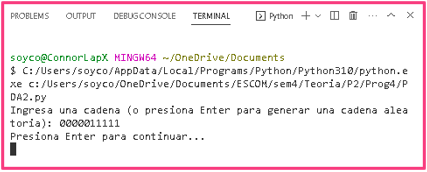
\includegraphics[width=4\linewidth]{Images/Cap1.png}
\end{minipage}
\caption{Inicio del programa en terminal.}
\label{fig:imagen}
\end{figure}
\newpage
\item Aquí se puede visualizar la animación del autómata pila. Se inserta X. Observar la Figura 2.2.\newline
\begin{figure}[h]
\begin{minipage}{0.3\textwidth}
    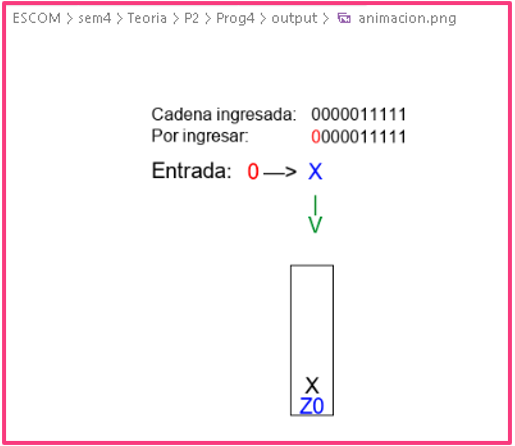
\includegraphics[width=3.5\linewidth]{Images/Cap2.png}
\end{minipage}
\caption{Animación primera parte.}
\label{fig:imagen}
\end{figure}

\newpage
\item Segunda parte de animación y terminal, se inserta X. Observar la Figura 2.3.
\begin{figure}[h]
%\begin{minipage}{0.3\textwidth}
    \begin{center}
    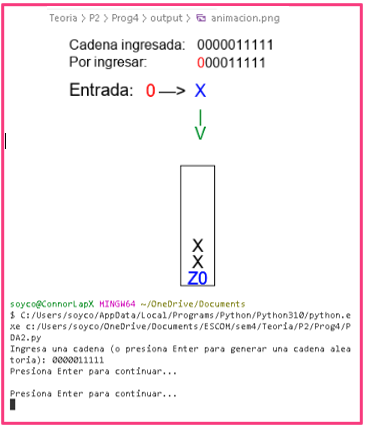
\includegraphics[width=0.7\linewidth]{Images/Cap3.png}
    \end{center}
%\end{minipage}
\caption{Segunda parte de animación y terminal.}
\label{fig:imagen}
\end{figure}

\newpage
\item Tercera parte de animación y terminal, se inserta X. Observar la Figura 2.4.
\begin{figure}[h]
%\begin{minipage}{0.3\textwidth}
    \begin{center}
    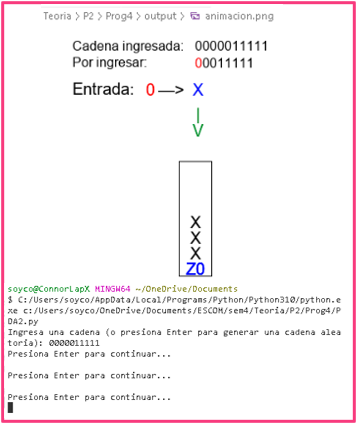
\includegraphics[width=0.7\linewidth]{Images/Cap4.png}
    \end{center}
%\end{minipage}
\caption{Tercera parte de animación y terminal.}
\label{fig:imagen}
\end{figure}

\newpage
\item Cuarta parte de animación y terminal, se inserta X. Observar la figura 2.5.

\begin{figure}[h]
%\begin{minipage}{0.3\textwidth}
    \begin{center}
    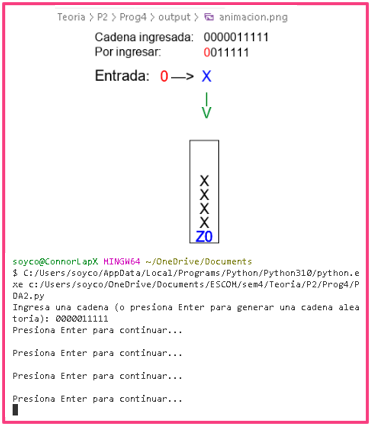
\includegraphics[width=0.7\linewidth]{Images/Cap5.png}
    \end{center}
%\end{minipage}
\caption{Cuarta parte de animación y terminal.}
\label{fig:imagen}
\end{figure}

\newpage
\item Quinta parte de animación y terminal, se inserta X. Observar la figura 2.6.

\begin{figure}[h]
%\begin{minipage}{0.3\textwidth}
    \begin{center}
    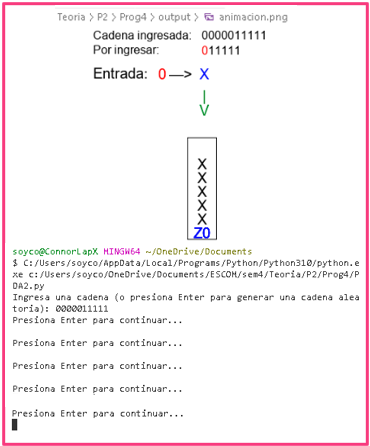
\includegraphics[width=0.7\linewidth]{Images/Cap6.png}
    \end{center}
%\end{minipage}
\caption{Quinta parte de animación y terminal.}
\label{fig:imagen}
\end{figure}
\newpage
\item Sexta parte de animación y terminal, se elimina X. Observar la figura 2.7.

\begin{figure}[h]
%\begin{minipage}{0.3\textwidth}
    \begin{center}
    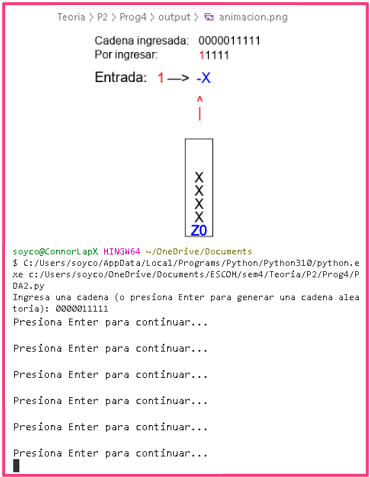
\includegraphics[width=0.7\linewidth]{Images/Cap7.png}
    \end{center}
%\end{minipage}
\caption{Sexta parte de animación y terminal.}
\label{fig:imagen}
\end{figure}
\newpage
\item Séptima parte de animación y terminal, se elimina X. Observar figura 2.8.

\begin{figure}[h]
%\begin{minipage}{0.3\textwidth}
    \begin{center}
    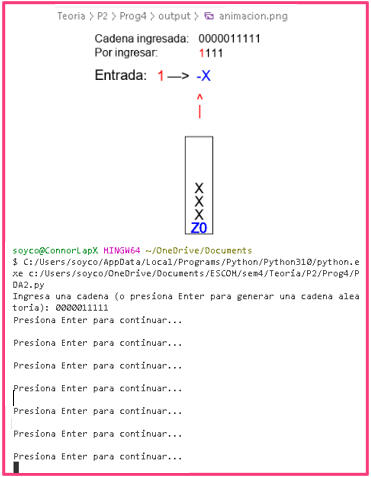
\includegraphics[width=0.6\linewidth]{Images/Cap8.png}
    \end{center}
%\end{minipage}
\caption{Séptima parte de animación y terminal.}
\label{fig:imagen}
\end{figure}

\newpage
\item Octava parte de animación y terminal, se elimina X. Observar figura 2.9.

\begin{figure}[h]
%\begin{minipage}{0.3\textwidth}
    \begin{center}
    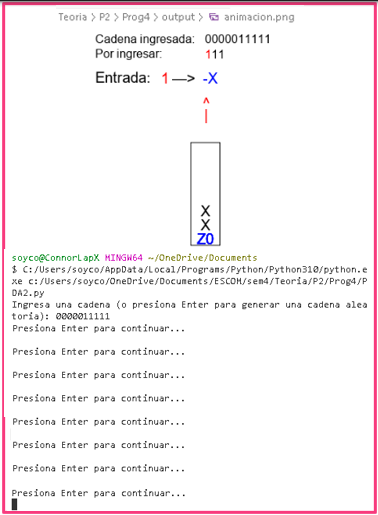
\includegraphics[width=0.6\linewidth]{Images/Cap9.png}
    \end{center}
%\end{minipage}
\caption{Octava parte de animación y terminal.}
\label{fig:imagen}
\end{figure}

\newpage
\item Novena parte de animación y terminal, se elimina X. Observar figura 2.10.

\begin{figure}[h]
%\begin{minipage}{0.3\textwidth}
    \begin{center}
    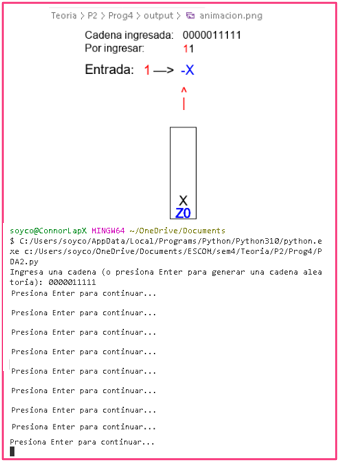
\includegraphics[width=0.6\linewidth]{Images/Cap10.png}
    \end{center}
%\end{minipage}
\caption{Novena parte de animación y terminal.}
\label{fig:imagen}
\end{figure}

\newpage
\item Décima parte de animación y terminal, se elimina X. Observar la figura 2.11.

\begin{figure}[h]
%\begin{minipage}{0.3\textwidth}
    \begin{center}
    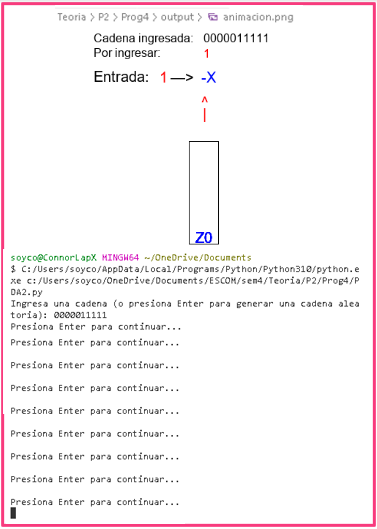
\includegraphics[width=0.6\linewidth]{Images/Cap11.png}
    \end{center}
%\end{minipage}
\caption{Décima parte de animación y terminal.}
\label{fig:imagen}
\end{figure}

\newpage
\item Onceava parte de animación y terminal, se recibe el vacío y, por lo tanto, se saca lo que haya en la pila, en este caso Z0. Observar la figura 2.12.

\begin{figure}[h]
%\begin{minipage}{0.3\textwidth}
    \begin{center}
    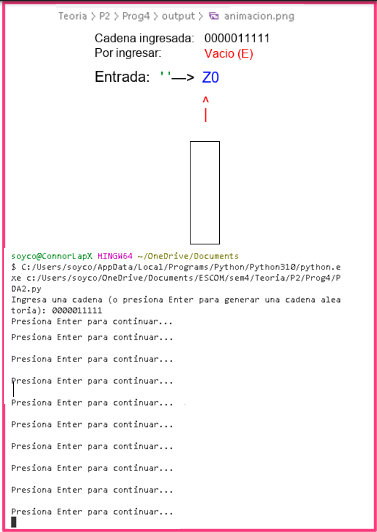
\includegraphics[width=0.6\linewidth]{Images/Cap12.png}
    \end{center}
%\end{minipage}
\caption{Onceava parte de animación y terminal.}
\label{fig:imagen}
\end{figure}

\newpage
\item Doceava parte de animación y terminal, se válida la cadena. Observar la figura 2.13.

\begin{figure}[h]
%\begin{minipage}{0.3\textwidth}
    \begin{center}
    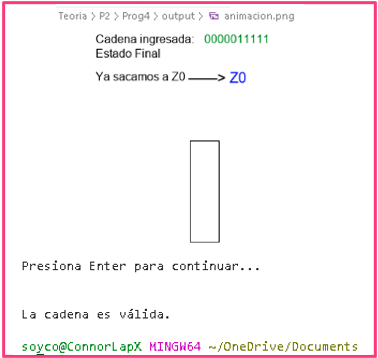
\includegraphics[width=0.6\linewidth]{Images/Cap13.png}
    \end{center}
%\end{minipage}
\caption{Doceava parte de animación y terminal.}
\label{fig:imagen}
\end{figure}
\newpage
\item Aquí podemos ver el archivo de salida de transiciones.txt, y poder visualizar como se llevó a cabo la construcción de la pila. Observar la figura 2.14.

\begin{figure}[h]
%\begin{minipage}{0.3\textwidth}
    \begin{center}
    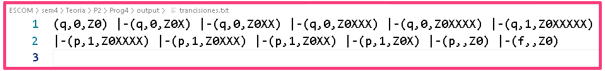
\includegraphics[width=1\linewidth]{Images/Cap14.png}
    \end{center}
%\end{minipage}
\caption{Archivo de salida de transiciones.txt.}
\label{fig:imagen}
\end{figure}
\newpage
\item En esta aparte pedimos al programa una cadena aleatoria presionando Enter, se digito aleatoriamente una cadena de tamaño 70,196. Observar la figura 2.15.

\begin{figure}[h]
%\begin{minipage}{0.3\textwidth}
    \begin{center}
    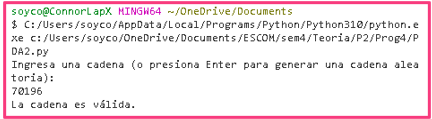
\includegraphics[width=1\linewidth]{Images/Cap15.png}
    \end{center}
%\end{minipage}
\caption{Nueva entrada aleatoria.}
\label{fig:imagen}
\end{figure}
\newpage
\item Aquí podemos ver el inicio del archivo de salida de transiciones.txt, y poder visualizar como se llevó a cabo la construcción de la pila. Observar la figura 2.16.

\begin{figure}[h]
%\begin{minipage}{0.3\textwidth}
    \begin{center}
    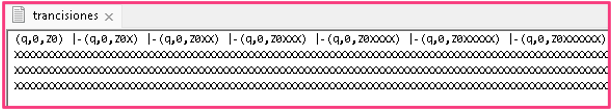
\includegraphics[width=1\linewidth]{Images/Cap16.png}
    \end{center}
%\end{minipage}
\caption{Inicio de archivo de trancisiones.txt.}
\label{fig:imagen}
\end{figure}
\newpage
\item Aquí podemos ver el final del archivo de salida de transiciones.txt, y poder visualizar como se llevó a cabo la construcción de la pila. Observar la figura 2.17.

\begin{figure}[h]
%\begin{minipage}{0.3\textwidth}
    \begin{center}
    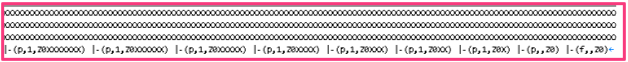
\includegraphics[width=1\linewidth]{Images/Cap17.png}
    \end{center}
%\end{minipage}
\caption{Final de archivo de trancisiones.txt .}
\label{fig:imagen}
\end{figure}
\end{enumerate}
\chapter{Conclusión}

Durante el desarrollo de este programa de autómata de pila, he logrado comprender en profundidad los conceptos relacionados con los lenguajes contextuales y su análisis. La implementación de este programa me ha permitido explorar la estructura y validación de lenguajes formales, así como comprender la importancia de las estructuras de datos en el análisis sintáctico.\newline

A través de esta experiencia, he aprendido cómo utilizar los autómatas de pila como herramienta fundamental en la teoría de la computación. Estos autómatas tienen una amplia gama de aplicaciones prácticas, como la compilación de lenguajes de programación, el análisis de lenguajes naturales y la verificación de la corrección sintáctica en diversos contextos.\newline
\\

\section{Problemas iniciales}
Durante el desarrollo del problema del autómata de pila, se presentaron algunos desafíos iniciales que requirieron atención y resolución. Estos problemas iniciales incluyeron:\newline
\begin{enumerate}
    \item Comprender el concepto de autómata de pila: Al inicio, fue necesario comprender en detalle qué es un autómata de pila y cómo funciona. Esto implicó estudiar su estructura, transiciones y comportamiento en la resolución de problemas de lenguajes formales.\newline

        
    \item Diseñar la estructura de datos adecuada: Para implementar el autómata de pila, fue necesario seleccionar una estructura de datos adecuada que permitiera representar y manipular la pila. Esto implicó evaluar diferentes opciones y elegir la más eficiente y conveniente para el problema en cuestión.\newline
    
    \item Definir las reglas de transición: El siguiente desafío fue establecer las reglas de transición del autómata de pila para cada símbolo de entrada. Esto requería comprender las reglas de la gramática y definir correctamente las transiciones en función de los símbolos de entrada y el estado actual del autómata.\newline
    
    \item Manejo de casos de error y ambigüedades: Durante la implementación, surgió la necesidad de manejar casos de error y ambigüedades en la entrada. Esto implicó considerar situaciones como símbolos no válidos, cadenas mal formadas o transiciones no definidas, y diseñar mecanismos para manejar estas situaciones de manera adecuada.\newline

\end{enumerate}


Enfrentar estos problemas iniciales y abordarlos de manera adecuada fue fundamental para el desarrollo exitoso del problema del autómata de pila. Cada uno de estos desafíos brindó oportunidades para aprender y fortalecer los conocimientos sobre teoría de la computación y lenguajes formales.




\newline

\subsection{Soluciones}
Se llevó a cabo un estudio detallado del autómata de pila para comprender su funcionamiento y aplicaciones relevantes. Posteriormente, se eligió una estructura de datos adecuada para representar la pila, garantizando eficiencia y facilidad de manipulación.\newline

Se definieron reglas de transición precisas para el autómata, considerando todos los estados, símbolos de entrada y las acciones correspondientes. Además, se implementaron mecanismos para manejar errores y ambigüedades en la entrada, asegurando la validez de los símbolos y la corrección en el procesamiento de las cadenas.\newline

Estas soluciones permitieron superar los desafíos iniciales y lograr una implementación exitosa del autómata de pila en el código proporcionado.\newline 
\section{Complejidades}
Supongamos que la longitud de la cadena de entrada es n. En el peor de los casos, el bucle while se ejecutará n + 1 veces, ya que también se ejecuta una vez más después de procesar todos los caracteres de la cadena.\newline 

Dentro del bucle, se realizan operaciones como comprobaciones de pertenencia en un diccionario ((estado\_actual, symbol, cima\_de\_pila) in PDA), acceso a elementos de diccionario (transiciones = PDA$[$(estado\_actual, symbol, cima\_de\_pila)$]$), operaciones de pila (pila.pop(), $pila.append(letra\_apuntada)$), concatenación de cadenas (''.join(pila)), y asignaciones de variables. Estas operaciones tienen una complejidad constante, es decir, no dependen del tamaño de la cadena de entrada.\newline 

Por lo tanto, la complejidad total de la función proceso\_recorrido sin graficar es lineal, O(n), donde n es la longitud de la cadena de entrada.
\chapter{Bibliografias}
\begin{enumerate}
    \item Hopcroft, J. E., Motwani, R., & Ullman, J. D. (2006). Introduction to Automata Theory, Languages, and Computation (3rd ed.). Addison-Wesley.\newline
    \item Sipser, M. (2012). Introduction to the Theory of Computation (3rd ed.). Cengage Learning.\newline
    \item Papadimitriou, C. H. (1997). Elements of the Theory of Computation. Prentice-Hall.\newline
    \item Linz, P. (2006). An Introduction to Formal Languages and Automata (4th ed.). Jones & Bartlett Learning.\newline
\end{enumerate}



%\textbf{Nota}: {\color{red}Revisar esta sugerencia de Segun:} %\href{https://github.com/INGEOTEC/RegionalEmbeddings}{FastText Word Embeddings for Spanish Language Variations} 


%[Objetivo: ]

\chapter{Anexos}
\lstset{
    language=C,
    basicstyle=\ttfamily\small\color{black},
    numbers=left,
    numberstyle=\tiny,
    stepnumber=1,
    numbersep=8pt,
    backgroundcolor=\color{white},
    showspaces=false,
    showstringspaces=false,
    showtabs=false,
    frame=single,
    rulecolor=\color{magenta},
    tabsize=2,
    captionpos=b,
    breaklines=true,
    breakatwhitespace=false,
    title=\lstname,
    escapeinside={\%*}{*)},
    keywordstyle=\color{blue},
    commentstyle=\color{red},
    stringstyle=\color{orange},
    morecomment=[l][\color{red}]{\#},
    otherkeywords={=,!,<,>,*,+,-,&,|,^,~},
    numbers=left,                   % Coloca los números de línea a la izquierda
    numberstyle=\tiny\color{black}, % Estilo de los números de línea
    stepnumber=1,    % Incremento en el que se muestran los números de línea
    numbersep=8pt
}
\section{PDA.py}
Se presenta el código implementado para la solución al problema con extensión .py . \newline
\\
\begin{lstlisting}
#Teoria de la computacion
#Automata de pila
#Alumno: Connor Urbano Mendoza

import random
from PIL import Image, ImageDraw,ImageFont
import sys

# Tamaño de la imagen y tamaño del cuadrado
image_size = (400, 400)
square_size = 100

# Crear una imagen en blanco
image = Image.new("RGB", image_size, "white")
draw = ImageDraw.Draw(image)



# Definir el PDA con sus transiciones
PDA = {
    ('q', '0', 'Z0'): [('q', 'X')],
    ('q', '0', 'X'): [('q', 'X')],
    ('q', '1', 'X'): [('p', '')],
    ('p', '1', 'X'): [('p', 'Z0')],
    ('p', '', 'Z0'): [('f', 'Z0')]
}

#Funcion de recorrido sin graficar
def proceso_recorrido(cadena,estado,i):
    ruta_archivo = "C:\\Users\\soyco\\OneDrive\\Documents\\ESCOM\\sem4\\Teoria\\P2\\Prog4\\output\\trancisiones.txt"
    with open(ruta_archivo, "w") as archivo:
        estado_actual=estado
        
        while i < (len(cadena)+1):
            if i == (len(cadena)):
                symbol=''
            else:
                symbol = cadena[i]
            cadena_pila = ''.join(pila)

            cima_de_pila = pila[-1]
            archivo.write("("+estado_actual+","+symbol+","+cadena_pila+") |-")
            if (estado_actual, symbol, cima_de_pila) in PDA:
                transiciones = PDA[(estado_actual, symbol, cima_de_pila)]
                estado_siguiente = transiciones[0][0]  
                letra_apuntada = transiciones[0][1]
                if(letra_apuntada == ''):
                    cima_de_pila = pila.pop()
                elif(letra_apuntada == 'Z0'):
                    cima_de_pila = pila.pop()
                else:
                    pila.append(letra_apuntada)
                    
                estado_actual=estado_siguiente
                i += 1
            else:
                archivo.write("Error")
                return False
        archivo.write("("+estado_actual+","+symbol+","+cadena_pila+")")    
        return True    
#Funcion de recorrido para graficar
def proceso_recorrido2(cadena,estado,i):
    
    ruta_archivo = "C:\\Users\\soyco\\OneDrive\\Documents\\ESCOM\\sem4\\Teoria\\P2\\Prog4\\output\\trancisiones.txt"
    with open(ruta_archivo, "w") as archivo:
        estado_actual=estado
        cadena_grafica = cadena
            
        while i < (len(cadena)+1):

            # Coordenadas del rectángulo
            rect_width = 40
            rect_height = 140
            x1 = ((image_size[0] - rect_width) // 2)
            desplazamientoa_abajo=60
            y1 = ((image_size[1] - rect_height) // 2) +desplazamientoa_abajo
            x2 = x1 + rect_width
            y2 = y1 + rect_height
            
            # Dibujar el rectángulo en la imagen
            draw.rectangle([(x1, y1), (x2, y2)], outline="black")
            #----------Dibujamos apartados-------------------------
            # Dibujamos apartados de cadena ingresada
            text = "Cadena ingresada:"
            font = ImageFont.truetype("arial.ttf", 16)

            # Dibujar el texto en la imagen
            draw.text((50, 40), text, fill="black", font=font)
            
            # Dibujar ecadenal texto en la imagen 
            draw.text((200, 40), cadena, fill="black", font=font) 
            
            
            # Dibujamos apartados de por ingresar
            text = "Por ingresar:"

            # Dibujar el texto en la imagen
            draw.text((50, 60), text, fill="black", font=font)
            
            #Dibujamos primer caracter
            j=0
            
            cadena_grafica = cadena_grafica[1:]  # Obtener la subcadena sin la primera letra
            draw.text((209, 61), cadena_grafica, fill="black", font=font)
            # Dibujamos apartados de entrada
            text = "Entrada:"
            font2 = ImageFont.truetype("arial.ttf", 20)

            # Dibujar el texto en la imagen
            draw.text((50, 90), text, fill="black", font=font2)
            
            #Coordenada de incremento para cruces
            cross_y = (((y1 + y2) // 2)+50) - ((i+1)*19)
            #Dibujamos caso base
            draw.text((189, (((y1 + y2) // 2)+50)), "Z0", fill="blue", font=font2)
            
            
            if i == (len(cadena)):
                symbol=''
                #Dibujamos primer caracter y la entrada
                # Dibujar el texto en la imagen
                draw.text((140, 91), "' '", fill="green", font=font2)
                draw.text((200, 61), "Vacio (E)", fill="red", font=font)
                #Dibujamos felcha de conversion
                draw.text((155, 91), "—>", fill="black", font=font2)
            else:
                symbol = cadena[i]
                number=int(symbol)
                # Dibujar el texto en la imagen
                draw.text((140, 91), symbol, fill="red", font=font2)
                draw.text((200, 61), symbol, fill="red", font=font)
                #Dibujamos felcha de conversion
                draw.text((155, 91), "—>", fill="black", font=font2)
                
            cadena_pila = ''.join(pila)
            cima_de_pila = pila[-1]
            
            archivo.write("("+estado_actual+","+symbol+","+cadena_pila+") |-")
            if (estado_actual, symbol, cima_de_pila) in PDA:
                transiciones = PDA[(estado_actual, symbol, cima_de_pila)]
                estado_siguiente = transiciones[0][0]  
                letra_apuntada = transiciones[0][1]
                if(letra_apuntada == ''):
                    cima_de_pila = pila.pop()
                    #Dibujamos letra
                    draw.text((197, 91), "-X", fill="blue", font=font2)
                    draw.text((197, 125), "^", fill="red", font=font2)
                    draw.text((199, 141), "|", fill="red", font=font2)
                    if len(cadena) % 2 != 0:
                        cross_y = ((((y1 + y2) // 2)+50) - ((i+1)*19)-19)
                    else:
                        cross_y = (((y1 + y2) // 2)+50) - ((i+1)*19)
                    # Coordenadas de la última cruz agregada
                    last_cross_x = 200
                    
                    last_cross_y = cross_y + ((38*i)-(19*len(cadena)))
                    last_cross_size = 12

                    # Guardar las coordenadas y el tamaño de la última cruz
                    last_cross_coords = [((last_cross_x - last_cross_size)-1, last_cross_y + 21), ((last_cross_x + last_cross_size)+1, (last_cross_y + 37)+1)]
                    # Eliminar la última cruz
                    draw.rectangle(last_cross_coords, outline="white", fill="white")
                    
                elif(letra_apuntada == 'Z0' and number==1 and symbol!=''):
                    cima_de_pila = pila.pop()
                    #Dibujamos letra
                    draw.text((197, 91), "-X", fill="blue", font=font2)
                    draw.text((197, 125), "^", fill="red", font=font2)
                    draw.text((199, 141), "|", fill="red", font=font2)
                    if len(cadena) % 2 != 0:
                        cross_y = ((((y1 + y2) // 2)+50) - ((i+1)*19)-19)
                    else:
                        cross_y = (((y1 + y2) // 2)+50) - ((i+1)*19)
                    # Coordenadas de la última cruz agregada
                    last_cross_x = 200
                    #print(cross_y)
                    last_cross_y = cross_y + ((38*i)-(19*len(cadena)))
                    last_cross_size = 12

                    # Guardar las coordenadas y el tamaño de la última cruz
                    last_cross_coords = [((last_cross_x - last_cross_size)-1, last_cross_y + 21), ((last_cross_x + last_cross_size)+1, (last_cross_y + 37)+1)]
                    # Eliminar la última cruz
                    draw.rectangle(last_cross_coords, outline="white", fill="white")
                elif(letra_apuntada == 'Z0' and symbol==''):
                    cima_de_pila = pila.pop()
                    #Dibujamos letra
                    draw.text((197, 91), "Z0", fill="blue", font=font2)
                    draw.text((197, 125), "^", fill="red", font=font2)
                    draw.text((199, 141), "|", fill="red", font=font2)
                    # Coordenadas de la última cruz agregada
                    last_cross_x = 200
                    #print(cross_y)
                    last_cross_y = cross_y + ((38*i)-(19*len(cadena)))
                    last_cross_size = 12

                    # Guardar las coordenadas y el tamaño de la última cruz
                    last_cross_coords = [((last_cross_x - last_cross_size)-1, last_cross_y + 21), ((last_cross_x + last_cross_size)+1, (last_cross_y + 37)+1)]
                    # Eliminar la última cruz
                    draw.rectangle(last_cross_coords, outline="white", fill="white")
                else:
                    pila.append(letra_apuntada)
                    #Dibujamos letra
                    draw.text((197, 91), letra_apuntada, fill="blue", font=font2)
                    draw.text((201, 121), "|", fill="green", font=font2)
                    draw.text((197, 141), "V", fill="green", font=font2)
                    #Dibujamos cruz
                    draw.text((194, cross_y), "X", fill="black", font=font2)
                    
                estado_actual=estado_siguiente
                
                # Guardar la imagen en la ruta especificada
                image.save("C:\\Users\\soyco\\OneDrive\\Documents\\ESCOM\\sem4\\Teoria\\P2\\Prog4\\output\\animacion.png")
                if sys.stdin.isatty():
                    print("Presiona Enter para continuar...")
                    sys.stdin.readline()
                else:
                    input("Presiona Enter para continuar...")
                i += 1
            else:
                archivo.write("Error")
                #Dibujamos letra
                # Cadena invalida
                draw.text((200, 40), cadena, fill="red", font=font) 
                draw.text((197, 91), "ERROR", fill="blue", font=font2)
                
                image.save("C:\\Users\\soyco\\OneDrive\\Documents\\ESCOM\\sem4\\Teoria\\P2\\Prog4\\output\\animacion.png")
                if sys.stdin.isatty():
                    print("Presiona Enter para continuar...")
                    sys.stdin.readline()
                else:
                    input("Presiona Enter para continuar...")
                return False
            
            # Aquí se realiza el borrado del contenido de la imagen
            draw.rectangle([(11, 11), (389, 180)], fill="white")
            image.save("C:\\Users\\soyco\\OneDrive\\Documents\\ESCOM\\sem4\\Teoria\\P2\\Prog4\\output\\animacion.png")

            
        archivo.write("("+estado_actual+","+symbol+","+cadena_pila+")")    
        
        # Coordenadas del rectángulo
        rect_width = 40
        rect_height = 140
        x1 = ((image_size[0] - rect_width) // 2)
        desplazamientoa_abajo=60
        y1 = ((image_size[1] - rect_height) // 2) +desplazamientoa_abajo
        x2 = x1 + rect_width
        y2 = y1 + rect_height
        
        # Dibujar el rectángulo en la imagen
        draw.rectangle([(x1, y1), (x2, y2)], outline="black")
        
        # Dibujamos apartados de cadena ingresada
        text = "Cadena ingresada:"
        font = ImageFont.truetype("arial.ttf", 16)

        # Dibujar el texto en la imagen
        draw.text((50, 40), text, fill="black", font=font)
        
        # Dibujar ecadenal texto en la imagen 
        draw.text((200, 40), cadena, fill="green", font=font) 
        
        text = "Estado Final"

        # Dibujar el texto en la imagen
        draw.text((50, 60), text, fill="black", font=font)
        
        # Dibujamos apartados de entrada
        text = "Ya sacamos a Z0"
        # Dibujar el texto en la imagen
        draw.text((50, 92), text, fill="black", font=font)
        #Dibujamos felcha de conversion
        draw.text((178, 91), "——>", fill="black", font=font2)
                
        
        draw.text((235, 91), "Z0", fill="blue", font=font2)
        
        image.save("C:\\Users\\soyco\\OneDrive\\Documents\\ESCOM\\sem4\\Teoria\\P2\\Prog4\\output\\animacion.png")
        if sys.stdin.isatty():
            sys.stdin.readline()
        else:
            input("Presiona Enter para continuar...")
        return True    

def generar_cadena_aleatoria(tamanio):
    mitad = tamanio // 2
    ceros = '0' * mitad
    unos = '1' * mitad
    if tamanio % 2 != 0:
        ceros += random.choice(['0', '1'])
    cadena = ceros + unos
    return cadena
    
    
#Main
pila = []

elemento_superior = 'Z0'
pila.append(elemento_superior)
estado = 'q'
i = 0

cadena = input("Ingresa una cadena (o presiona Enter para generar una cadena aleatoria): ")

if not cadena:
    tamanio = random.randint(1, 100000)
    print(tamanio)
    cadena = generar_cadena_aleatoria(tamanio)
    resultado = proceso_recorrido(cadena, estado, i)

    if resultado:
        print("La cadena es válida.")
    else:
        print("La cadena no es válida.")
    
else:
    resultado = proceso_recorrido2(cadena, estado, i)

    if resultado:
        print("La cadena es válida.")
    else:
        print("La cadena no es válida.")
    
\end{lstlisting}

Se presenta el código LaTeX de este archivo mediante el siguiente link:\newline
\\
Link overleaf: $"$\url{https://www.overleaf.com/read/tpnhwgwdrprq}$"$\newline
Link github: $"$\url{https://github.com/Connor-UM-18/Teoria-computacional-PDA.git}$"$\newline



%\bibliographystyle{apacite}
%\bibliography{References/predoc.bib}

\backmatter%@sglvgdor


\end{document}
